% Chapter Template

\chapter{Methodology} % Main chapter title
\label{chapter3} 

The following chapter includes methodological procedures that are common for all chapters.
More detailed methodological procedures will be described in each chapter separately. 

\section{Data}

We already briefly presented the datasets in the first chapter in section \ref{sec:data}.
Here, we will do an in-depth presentation of the datasets and present how we processed and cleaned the data. 

\subsection{Dataset selection}

The Table \ref{tab:other_datasets} was published on the NILMTK \cite{nilmtk} wiki page. 
NILMTK is a tool developed by authors in paper \cite{nilmtk}.
It intends to make the development of NILM algorithms easier by standardizing a format in which building energy consumption datasets are stored. 
They also developed converters to convert existing datasets into a universal format.
This enables engineers to simply load and process multiple datasets.
NILMTK includes a dataset converter from most of the datasets from table \ref{tab:other_datasets}.
\begin{table}[H]
    \centering
    \caption{Pruned version of the Table published by authors on NILMTK\protect{\cite{nilmtk}} wiki page. Full table available here \protect{\url{https://web.archive.org/web/20190607094329/http://wiki.nilm.eu/datasets.html}}.}
    \resizebox{\textwidth}{!}{\begin{tabular}{|l|l|l|l|l|l|l|l|l|}
    \hline
        \textbf{Dataset} & \textbf{Sampling rate} & \textbf{Duration } & \textbf{ Buildings } & \textbf{Subject} & \textbf{Country} & \textbf{Availability} \\ \hline
        Dataport & 1 Hz to 1 minute & 4+ years & 1200 & multiple & US & Licensed \\ \hline
        BLOND-50  & 50 kHz/6.4kHz & 213 days & 1 & office & Germany & Public \\ \hline
        FIRED & 12 kHz to 1 Hz & 101 days & 1 & residential & Germany & Public \\ \hline
        REDD & 16500 Hz / 1 Hz & 100 days & 5 & Residential & US & Request access \\ \hline
        BLUED & 12000 Hz & 7 days & 1 & Residential & US & Request access \\ \hline
        UK-DALE & 16000 Hz / 1 Hz & 2 years & 6 & Residential & UK & Public \\ \hline
        PLAID & 30000 Hz & 5 seconds & 55 & Appliances & US & Public \\ \hline
        WHITED & 44000 Hz & 5 seconds & 9 & Appliances & Multiple & Public \\ \hline
        Tracebase & 1 Hz & 1 day & 158 & Appliances & Germany & Request access \\ \hline
        DRED & 1 Hz / 1 min & 150 days & 1 & Residential & Netherlands & Public \\ \hline
        AMPds & 1 minute & 2 years & 1 & Residential & Canada & Public \\ \hline
        RAE & 1 Hz & 72 days & 1 & Residential & Canada & Public \\ \hline
        iAWE & 1 Hz & 73 days & 1 & Residential & India & Public \\ \hline
        HES & 2 minutes & 1 year & 251 & Residential & UK & Request access \\ \hline
        REFIT & 8 seconds & 2 years & 20 & Residential & UK & Public \\ \hline
        ECO & 1 second & 200 days & 6 & Residential & Switzerland & Public \\ \hline
        COMBED & 30 seconds & 30 days & ~ & Office & India & ~ \\ \hline
        IHEPCDS & 1 minute & 4 years & 1 & ~ & France & ~ \\ \hline
        SMART & 1 Hz & 60 days & 3 & ~ & USA & ~ \\ \hline
        LIT-Dataset & 15 kHz & 30 seconds & 26 & Residential & Brazil & Public \\ \hline
    \end{tabular}}
    \label{tab:other_datasets}
\end{table}

The reason why more datasets were not selected from the Table \ref{tab:other_datasets},
was because we followed the criteria:
\begin{enumerate}
    \item Sampling rate between 1 Hz and 1/10 Hz
    \item Duration more than 30 days
    \item Subject had to be a residential area building
    \item Include main meter as well as sub-meter measurements
    \item Has to be accessible
\end{enumerate}

After applying these criteria we were left with the following datasets:

\begin{itemize}
    \item UK-DALE \cite{UKDALE}
    \item REFIT \cite{REFIT}
    \item ECO \cite{ECO}
    \item REDD \cite{REDD}
    \item iAWE \cite{iAWE}.
\end{itemize}

\subsection{Processing}
After datasets were obtained and converted they were ready to be processed.
We decided to slice the data into hourly slices so that it will be easier to find missing data and build LPs.

Firstly we resampled the time series data  1/6 Hz. 
This had to be done since datasets were sampled at different frequencies.
A frequency of 1/6 Hz is commonly used since it has a good ratio between resource usage and NILM algorithm performance.
Resampling was done using Pandas resample. 
We used a forward fill parameter with a limit of 5.
This means that in case of missing data, we will fill in no more than 5 samples, with the last known value.
Secondly, we sliced the time series data into hourly slices. 
With one sample every 6 seconds, there were roughly 60 samples in every slice.
Thirdly, we removed slices with missing data.
This was done for all slices where there was more than 20 \% of data missing.
In cases where less than 20 \% of data was missing, we forward-filled it with the last known value.
In the worst case, we forward filled 12 samples. 
Finally, resampled and cleaned data was stored in the following manner.
\begin{verbatim}
   /dataset/appliance/building/
\end{verbatim}

\subsection{Training and health}

\subsection{Datasets and evaluation} \label{ssec:ds_eval}

The data was split into train and test sets, where 80 \% of the data was used for training and 20 \% percent of the data for testing.
The data was split based on the number of samples, so in some cases where there is a lot of missing data, the time window of test data might be longer, although it contains only 20 \% of the samples.

\subsubsection{REFIT}
The REFIT \cite{REFIT} dataset included data for more than 15 buildings, as can be seen in the Figure below.
The dataset in general is of the highest quality since it is the longest with the least missing data.
This means this dataset should give the most relevant results.
\begin{figure}[H]
	\centering
	\caption{Timeline for REFIT}
	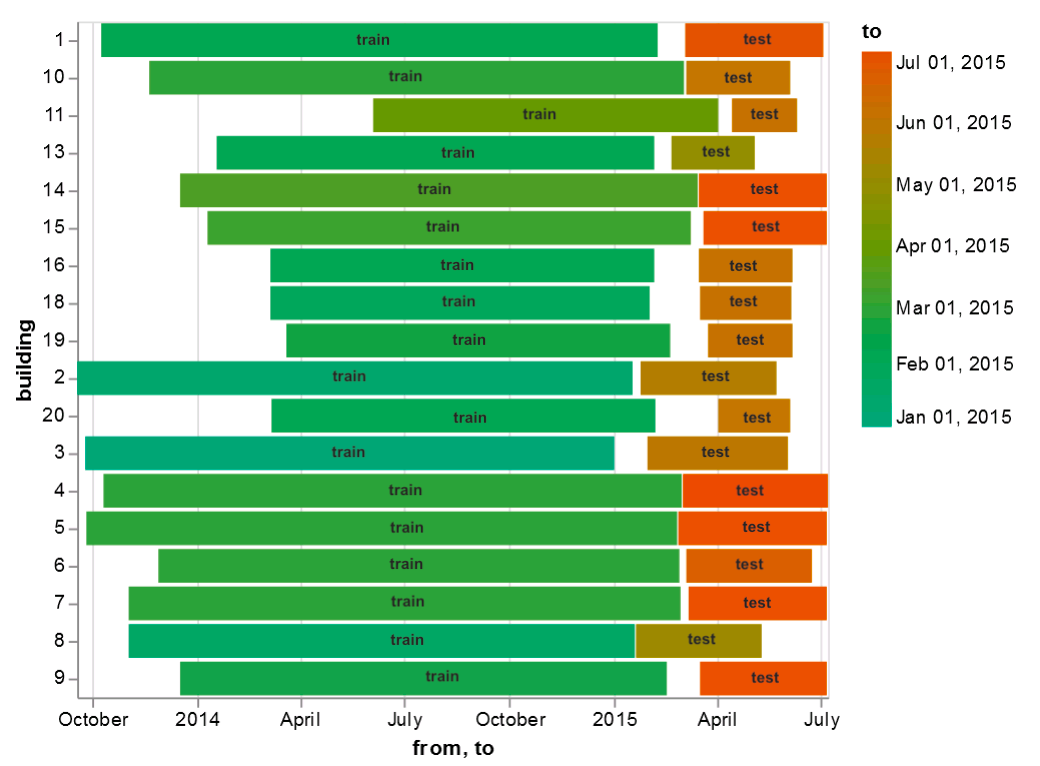
\includegraphics[width=1\textwidth]{Figures/EC/refit_timeline.png}
	\label{fig:refit_timeline}
\end{figure}

\subsubsection{UK-DALE} 

Through the UK-DALE \cite{UKDALE} dataset is of similar size, most of the data is from building 1.
In general, it includes 5 years of data, but only for some appliances, where many appliances are rarely used.
When taking all of this into account, there were too many issues with building 1, and it was simply ignored.
Another issue that can be seen in Figure \ref{fig:ukdale_timeline} is that there is not enough data for 
building 3. The test includes only a week of data, which is not enough for representative results, therefore it was ignored.
The rest of the buildings seem healthy.

\begin{figure}[H]
	\centering
	\caption{Timeline for UK-DALE}
	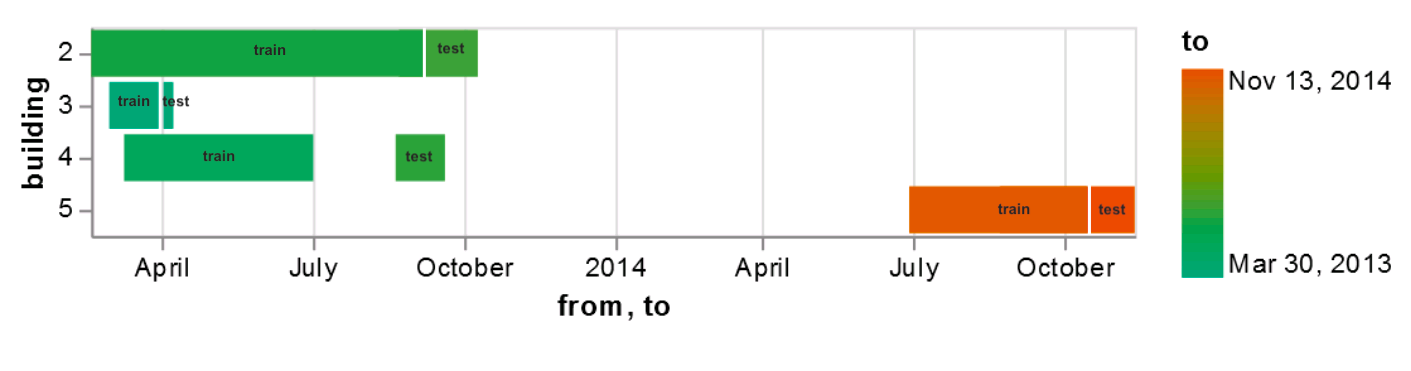
\includegraphics[width=1\textwidth]{Figures/EC/ukdale_timeline.png}
	\label{fig:ukdale_timeline}
\end{figure}

\subsubsection{ECO}
ECO \cite{ECO} dataset has a length of data similar to UK-DALE. 
The only issue is building 1, where there is a lot of missing data.
This is a good example of how data is split, it is split based on several samples,
meaning that there is 80 \% in the train bar, due to missing data the second bar is longer. 

\begin{figure}[H]
	\centering
	\caption{Timeline for ECO}
	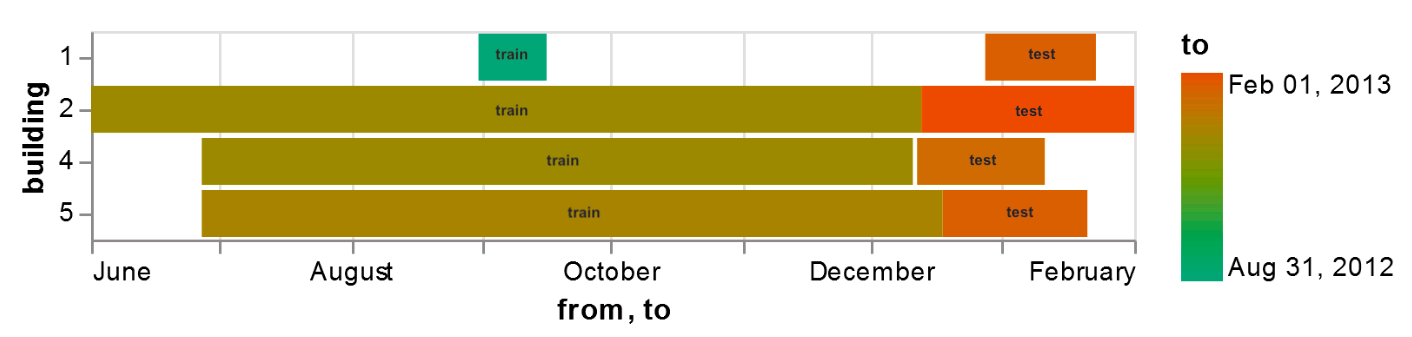
\includegraphics[width=1\textwidth]{Figures/EC/eco_timeline.png}
	\label{fig:eco_timeline}
\end{figure}


\section{Tools Used}



To process the data and to obtain the results the environment and virtual machines from Google Colab \cite{colab} were used.
They offer access to Google GPU-accelerated compute machines with 12 GB of RAM. 
Colab also offers access to Drive cloud storage, where the dataset and results were stored.
While running the experiments, we made use of Drives 100 TB pooled cloud storage, which is available to students of the University of Ljubljana. 
For development and version control, GitHub was used. 

Within the Colab which uses a Jupyter \cite{jupyter} environment at its core, various python libraries were used.
To store and read the datasets in hdf5 format we used h5py  \cite{hdf5} and Pickle  \cite{pickle}.
To load datasets into RAM and then handle them, the pandas  \cite{pandas} library was used.
For handling the large matrices and calculating we used NumPy  \cite{numpy}.
To present the data with graphs we have used Matplotlib  \cite{matplotlib} and to present data with heatmap Seaborn  \cite{seaborn}.
For easier implementation, such as of the t-SNE, a Scikit  \cite{scikit} and SciPy  \cite{scipy} libraries were used.
